Uno de los principales objetivos de SNMP es permitir la supervisión continua del estado operativo de una infraestructura informática. Mediante la recopilación periódica de información desde múltiples agentes distribuidos en la red, un sistema de gestión puede construir una visión global del estado de un cluster de servidores, detectar anomalías y generar alertas antes de que los problemas afecten a los servicios ofrecidos.

La combinación entre SNMP y las distintas MIBs estandarizadas permite acceder a métricas de red, recursos de hardware y parámetros del sistema operativo utilizando una interfaz uniforme e independiente del fabricante.

\subsection{Métricas Clave a Monitorizar}

La monitorización efectiva de un cluster requiere observar tanto el estado de la red como los recursos internos de cada nodo. Las métricas recopiladas permiten identificar cuellos de botella, tendencias de crecimiento y posibles fallos de hardware.

\subsubsection{Uso de CPU}

La utilización del procesador constituye uno de los indicadores más importantes del estado de un servidor. Valores elevados de uso sostenido pueden indicar sobrecarga de aplicaciones, problemas de planificación de procesos o falta de capacidad computacional.

En entornos de monitorización, esta información suele obtenerse mediante objetos definidos en la HOST-RESOURCES-MIB y otras extensiones específicas del sistema operativo.

\subsubsection{Memoria RAM}

El consumo de memoria permite determinar si un sistema dispone de recursos suficientes para ejecutar sus aplicaciones. La falta de memoria disponible puede provocar intercambio excesivo con disco (\textit{swapping}) y degradar significativamente el rendimiento general del servidor.

El seguimiento continuo de este parámetro facilita la planificación de capacidad y la detección temprana de problemas de dimensionamiento.

\subsubsection{Almacenamiento e I/O de Disco}

Los subsistemas de almacenamiento representan otro componente crítico dentro de un cluster. La monitorización del espacio disponible, el rendimiento de lectura y escritura, así como el estado de los dispositivos físicos, permite anticipar fallos y evitar interrupciones del servicio.

En infraestructuras modernas, esta información suele complementarse con MIBs propietarias proporcionadas por fabricantes de controladoras y sistemas de almacenamiento.

\subsubsection{Tráfico de Red}

Las interfaces de red generan una gran cantidad de información estadística accesible mediante IF-MIB y MIB-II.

Entre las métricas más utilizadas se encuentran:

\begin{itemize}
\item Bytes transmitidos y recibidos.
\item Utilización de enlaces.
\item Paquetes descartados.
\item Errores de transmisión.
\item Retransmisiones TCP.
\end{itemize}

Estos indicadores permiten detectar congestión, fallos físicos y degradación de enlaces dentro del cluster.

\subsubsection{Temperatura y Estado de Hardware}

Los servidores modernos incorporan sensores que permiten supervisar temperatura, velocidad de ventiladores, fuentes de alimentación redundantes y otros componentes críticos.

Esta información suele encontrarse disponible mediante MIBs propietarias asociadas a plataformas de administración remota como Dell iDRAC, HP iLO o Cisco UCS.

La monitorización de estos parámetros resulta fundamental para prevenir fallos físicos y reducir el riesgo de interrupciones inesperadas.

\subsubsection{Disponibilidad del Sistema}

Una métrica ampliamente utilizada es \textit{sysUpTime}, que indica el tiempo transcurrido desde el último reinicio del dispositivo.

Cambios inesperados en este valor pueden revelar reinicios no planificados, fallos de hardware o problemas de estabilidad del sistema operativo.

\begin{figure}[H]
\centering
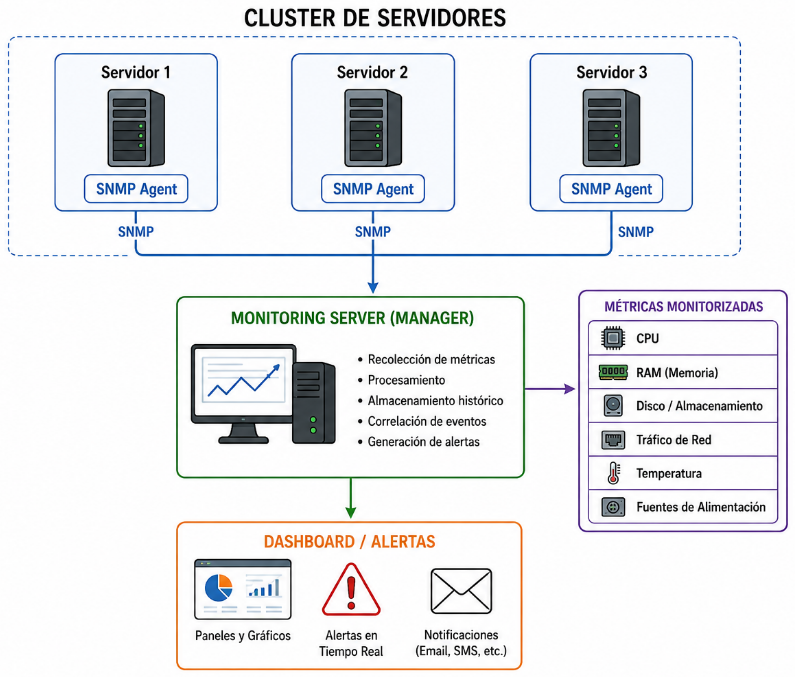
\includegraphics[width=0.85\textwidth]{img/snmp5.png}
\caption{Principales métricas monitorizadas mediante SNMP en un cluster de servidores.}
\label{fig}
\end{figure}

\subsection{SNMP Traps para Alertas en Tiempo Real}

Aunque el mecanismo de polling proporciona una visión periódica del estado de la infraestructura, muchas situaciones requieren una respuesta inmediata.

Para resolver esta limitación, SNMP incorpora mecanismos de notificación asíncrona basados en mensajes \textit{Trap} e \textit{InformRequest}.

Los agentes pueden generar alertas automáticamente cuando detectan eventos relevantes, evitando que el sistema de gestión tenga que esperar hasta la próxima consulta programada.

Entre los eventos más comunes se encuentran:

\begin{itemize}
\item Caída de interfaces de red.
\item Reinicios del dispositivo.
\item Fallos de autenticación.
\item Errores de hardware.
\item Superación de umbrales configurados.
\end{itemize}

Este mecanismo permite implementar estrategias de monitorización proactiva, reduciendo significativamente el tiempo necesario para detectar y responder a incidentes.

\subsection{Integración con Sistemas de Monitoreo}

En una arquitectura de monitorización moderna, SNMP actúa como mecanismo de adquisición de datos, mientras que plataformas especializadas procesan, almacenan y visualizan la información recopilada.

Desde el punto de vista conceptual, estas plataformas cumplen el rol de \textit{Manager}, interactuando con múltiples agentes distribuidos en la infraestructura.

Entre las funcionalidades habitualmente proporcionadas por estas herramientas se encuentran:

\begin{itemize}
\item Recolección periódica de métricas.
\item Almacenamiento histórico de datos.
\item Generación automática de alertas.
\item Correlación de eventos.
\item Visualización mediante paneles de control.
\item Elaboración de informes de capacidad y disponibilidad.
\end{itemize}

En entornos empresariales es habitual integrar SNMP con plataformas de monitorización como Nagios, Zabbix, Prometheus mediante exportadores compatibles y herramientas de visualización como Grafana.

Estas soluciones permiten transformar los datos obtenidos desde las MIBs en indicadores operativos comprensibles para administradores y equipos de operaciones.

\subsection{Importancia de SNMP en la Gestión de Clusters}

La principal ventaja de SNMP en entornos de clusters radica en su capacidad para proporcionar una visión unificada de múltiples nodos utilizando una interfaz estandarizada.

Gracias a la combinación de MIBs estándar y extensiones propietarias, los sistemas de gestión pueden supervisar simultáneamente recursos de red, sistemas operativos y componentes físicos de distintos fabricantes.

Esta capacidad de integración, junto con su amplia adopción en la industria, explica por qué SNMP continúa siendo una de las tecnologías fundamentales para la operación y monitorización de centros de datos modernos.